\documentclass[12pt]{article}
\usepackage[utf8]{inputenc}
\usepackage[a4paper, total={6.5in, 9.5in}]{geometry}
\usepackage{amsmath}
\usepackage{graphicx}
\usepackage{setspace}
\usepackage[autocite = superscript]{biblatex}
\addbibresource{Mendeley.bib}
\usepackage[compatibility=false]{caption}
\usepackage{subcaption}
\usepackage[section]{placeins}
\usepackage{enumitem}
\setlist[itemize]{noitemsep, topsep=0pt}
\setlist[enumerate]{noitemsep, topsep=0pt}

\renewcommand{\rmdefault}{ptm}
\usepackage[compact]{titlesec}
\titleformat{\section}[runin]{\normalfont\bfseries}{}{0pt}{}[\kern 1pc]
\titlespacing*{\section}{0pt}{0pt}{0pt}

\usepackage{footmisc}

\title{NSF GRFP Research Statement}
\author{Matthew Moreno}

\begin{document}
\begin{center}
{
 \textbf{Selecting for Irregular Refinement Potential in Evolving Artificial Neural Networks}
}
\end{center}
\vspace{-2.2ex}

\section{Summary}
Artificial Neural Networks (ANNs) have provided computational means to address previously intractable tasks such as image classification and automated language translation.
ANNs with high potential for irregular refinement (HPFIR ANNs) are highly desirable because they serve as a springboard for existing techniques such as direct-encoded evolutionary search or backpropagation.
This project will investigate how phenotypic plasticity might bias evolutionary search toward networks with high potential for irregular refinement.
This work aims to develop methodology to evolve such networks.


\section{Background}

Neuroevolution aims to design artificial neural network (ANN) topologies and weighting schemes through repeated evaluation, selection, and recombination of candidate solutions, an algorithm inspired by biological evolution. In the biological metaphor, candidate solutions have a phenotype, an ANN configuration that evolutionary selection acts upon, and a genotype, information that mutation and recombination act on and from which the phenotype is constructed. Genotypic representations are said to be either direct, indicating that each characteristic of the phenotype is stored verbatim in the genome, or indirect, indicating that the phenotype is generated from information that does not bear a one-to-one relationship to phenotypic characteristics. Direct mappings, which allow evolution to tweak individual phenotypic characteristics of candidate solutions independently, alllow fine-tooothed exploration of the phenotypic search space. Conversely, indirect genetic encodings, where genetic information is expanded via a process that allows for reuse of that information to uniformly describe a large number of phenotypic characteristics, has been demonstrated to bias evolutionary search towards phenotypic regularity\autocite{Clune2011OnRegularity}.

As a result of this bias, in highly regular problem domains evolutionary search with indirect genetic encoding outperforms search relying upon direct genetic encoding \autocite{Clune2011OnRegularity}. Nevertheless, most problem domains exhibit some irregularity, which often can only be exploited irregular phenotypic refinement; experimental evidence indicates that champion solutions evolved with indirect genetic encoding can often be bettered by irregular refinement vis-\`a-vis further evolutionary search with a direct encoding \autocite{Clune2011OnRegularity}. Clune et al. postulate that learning (post-developmental phenotypic plasticity of a neural network) similarly constitutes irregular refinement, enhancing the performance of a highly regular indirectly encoded phenotype via irregular modifications. Further, by allowing a candidate solution to assume proximal phenotypic forms, learning enables evolutionary selection to act on information about a candidate solution's local phenotypic neighborhood. Through selective pressure for phenotypes proximal to high-fitness phenotypic forms, local phenotypic search ``buys evolutionary time'' until heritable scaffolding arises to support phenotypic adaptation originally attained via plasticity \autocite{Downing2010TheNetworks}. This concept is termed the Baldwin effect.

\section{Motivation}

While neural architectures with high potential for irregular refinement are highly desirable, directly selecting for irregular refinement potential by performing complete irregular refinement on all candidate solutions is computationally prohibitive.
In the spirit of the Baldiwn effect, I propose that local phenotypic search via mutation to the direct representation of candidate solutions could bias evolutionary search toward neural architectures with high potential for irregular refinement.
While experimental results validate the Baldwin hypothesis,\autocite{Downing2009ComputationalEffect} the type and degree of local phenotypic search necessary to meaningfully bias evolutionary search is unknown.
The proposed research will characterize evolutionary bias towards artificial neural architectures with high irregular refinement potential induced by varied methods of local phenotypic search, specifically considering (1) the organization of local phenotypic search, the degree to which that search is biased by distribution of fitness over the local phenotypic space, and (2) selective preference for characteristics of local phenotypic space, the degree to which the presence of fitness peaks is considered over the overall fitness of the local phenotypic neighborhood.
A better understanding of these questions will translate to methodology that promotes evolution of neural architectures highly conductive to irregular refinement as well as furthering the theoretical conception of the interplay between phenotypic plasticity and evolution.
 


\section{Implementation}

Under the NGS regime, candidate solutions will consist of two components:
\begin{enumerate*}[label=(\arabic*)]
\item a raw architectural configuration $A$, and
\item a vector $v$ of network pruning parameters.
\end{enumerate*}
These components will be encoded and recombined separately using standard neuroevolution and genetic algorithm techniques, respectively.
To evaluate a candidate solution, the connection weights of the raw architectural configuration $A$ will be trained for a fixed number of iterations.
Then, a pruning decision will be made for each network node by comparing a quadratic weighting (defined by $v$) of the following metrics to a fixed cutoff value (also defined by $v$):
\begin{enumerate*}[label=(\alph*)]
\item node activation,
\item correlation of node activation with activation of afferent nodes,
\item correlation of node activation with loss, and
\item magnitude and sign of backpropagation gradient through the node.
\end{enumerate*}
Following pruning, training will resume for a fixed number of iterations. Candidate solution fitness will be assessed as the validation set performance of the final trained network.

\section{Research Plan}

I will investigate NGS in evolutionary deep learning architecture design in two stages.
First, in smaller scale experiments, I will compare evolvability and irregular refinement metrics under NGS and control treatments. Subsequently, in larger scale experiments, I will demonstrate the utility of NGS on benchmark deep learning datasets.
These experiments will be performed at the High Performance Computing Center at Michigan State University.

Small scale experiments will employ the HyperNEAT encoding,\autocite{clune2011performance} a standard indirect encoding for neuroevolution.
A variant of the bit mirroring problem, which is designed to permit explicit manipulation of problem regularity, will be employed.
Evolvability will be assessed by measuring the phenotypic novelty and viability of mutant offspring of champion candidate architectures.
The capacity of NGS-HyperNEAT to enable irregular refinement will be assessed by comparing control and NGS-HyperNEAT treatment performance across a spectrum of problem regularities.
Greater relative performance of NGS-HyperNEAT at low problem regularity would confirm that NGS enables irregular refinement.

Larger scale experiments will employ the CoDeepNEAT encoding,\autocite{miikkulainen2017evolving} an indirect encoding developed especially for evolving deep learning architectures.
Unlike HyperNEAT, the node-level unit in CoDeepNEAT is an ANN layer (instead of an individual neuron).
I will benchmark NGS-CoDeepNEAT on datasets for computer vision (CIFAR-10/100) and language modeling (PTB).
I expect performance to meet or exceed state-of-the-art.


\section{Expected Results}
Observation of evolutionary pressure for irregular refinement potential would suggest that the local phenotypic environment is predictive of irregular refinement potential.
If the elitist local search scheme yields solutions with high irregular refinement potential, then irregular refinement potential of an individual would ostensibly be correlated with phenotypes that are proximal to higher-fitness peaks in the phenotype space.
Similarly, evolution of solutions with high irregular refinement potential by the representative local search scheme would indicate that irregular refinement potential is correlated with phenotypes that have uniformly highly-fit neighbors.
Observing no effect of phenotypic plasticity on evolutionary bias towards irregular refinement potential would suggest that this potential might instead be associated with more diffuse properties of the phenotype space, a possibility that would warrant further investigation.


\section{Intellectual Merit}
By considering irregular refinement as a model of learning, this research applies an existing toolkit (based on the work of Clune et al.) to probe a poorly characterized theoretical construct: the Baldwin effect; it represents a novel link between to previously separate lines of EANN research \autocite{Clune2011OnRegularity,Downing2010TheNetworks}.
Further, this research has the potential to inform current efforts to understand what characteristics make neural architectures amenable to learning (both via local learning rules and backpropagation) and to develop methodology to evolve those network configurations.

Given the interdisciplinary nature of EANN research, experimental results of this project will be of interest to a wide variety scholarly circles.
It is especially pertinent to evolutionary biology, which is grappling with the role of phenotypic plasticity in evolution theory (among several contentious issues) as it undergoes a paradigm shift in evolution theory from the Modern Synthesis to the Extended Evolutionary Synthesis\autocite{Pigliucci2008IsEvolvable}.
Results describing evolutionary bias induced by representative and elitist models of phenotypic plasticity will directly inform these important conversations.


% \begin{itemize}
%   \item implications to broad questions of learning in EANN, the ultimate goal is to develop plastic EANN capable of on-line modification
%   \item
%   \item interdisciplinary: bridge gap between evolutionary biology and computer science
%   \item advances in EANN can bridge back to inform/expand our understanding of the evolutionary process \autocite{MoczekTheInnovation} \autocite{Pigliucci2008IsEvolvable} and emergent intelligence (i.e. neuroscience) in vivo
%   \item ``Extended Evolutionary Synthesis'' ``The broader context is that evolvability will constitute one of the foundational blocks for the much anticipated (or dreaded) EES in evolutionary biology93, together with other concepts that are new to — and yet build upon the achievements of — the Modern Synthesis.
% This expan- sion will include the role of phenotypic and behavioural plasticity 4,7, a better understanding of the evolution of develop- ment8–13, the role of epigenetic inheritance systems94, the idea of genetic accommoda- tion7, the dynamics of evolution in highly dimensional adaptive landscapes57, and of course the wealth of information provided by the post-genomic era95.
% It is an exciting moment to be an evolutionary biologist.'' \autocite{Pigliucci2008IsEvolvable}
%   \item The Baldwin effect postulates that network plasticity can pave the way for heritable variation \autocite{Downing2009ComputationalEffect}
%   \item Baldwin effect and learning: the most naive version; how much sophistication is required in the learning process to observe this effect
% \end{itemize}


\section{Broader Impact}

This research will contribute to the march of EANN towards networks with the size and plasticity rivaling those of their biological counterparts \cite{Clune2011OnRegularity,Tonelli2013OnNetworks}. This research is especially applicable in terms of evolving EANN that can take advantage of potential for lifetime irregular refinement. As EANN become more capable and the cost of parallel computing power continues to decrease, the EANN will become ripe for applications in the technology sector. Commercial pioneers, such as the recently founded Sentient Technologies, are already employing . This means that consumers benefit from the unique capabilities offered by EANN. In particular, the capability to train networks to do complex tasks that are not well suited to supervised learning and the potential for online learning in these systems  \cite{Downing2015IntelligenceSystems} means the potential for systems that can interface socially with people. The disruptive products are difficult to predict, but they will surely have a massive lifestyle impact.

\begin{itemize}
  \item artificial intelligence has direct applications to technology; stronger artificial intelligence has the potential to allow people to more fully exercise their human capacities
  \item EANN techniques are starting to be used in industry (i.e. Sentient AI)
  \item need to be more specific...
\end{itemize}

{\setstretch{0.9}
\begin{footnotesize}
\section{References}
\cite{Clune2011OnRegularity} \fullcite{Clune2011OnRegularity},
\cite{Downing2010TheNetworks} \fullcite{Downing2010TheNetworks},
\cite{Downing2009ComputationalEffect} \fullcite{Downing2009ComputationalEffect},
\cite{Hintze2017Mabe} \fullcite{Hintze2017Mabe},
\cite{Laland2014DoesRethink} \fullcite{Laland2014DoesRethink},
\cite{Mengistu2016EvolvabilityIt} \fullcite{Mengistu2016EvolvabilityIt}
\end{footnotesize}
\par}


%\section{Appendix}

\begin{figure}[!htbp]
   \centering
     \hfill
    \begin{subfigure}[b]{0.4\textwidth}
        \centering
        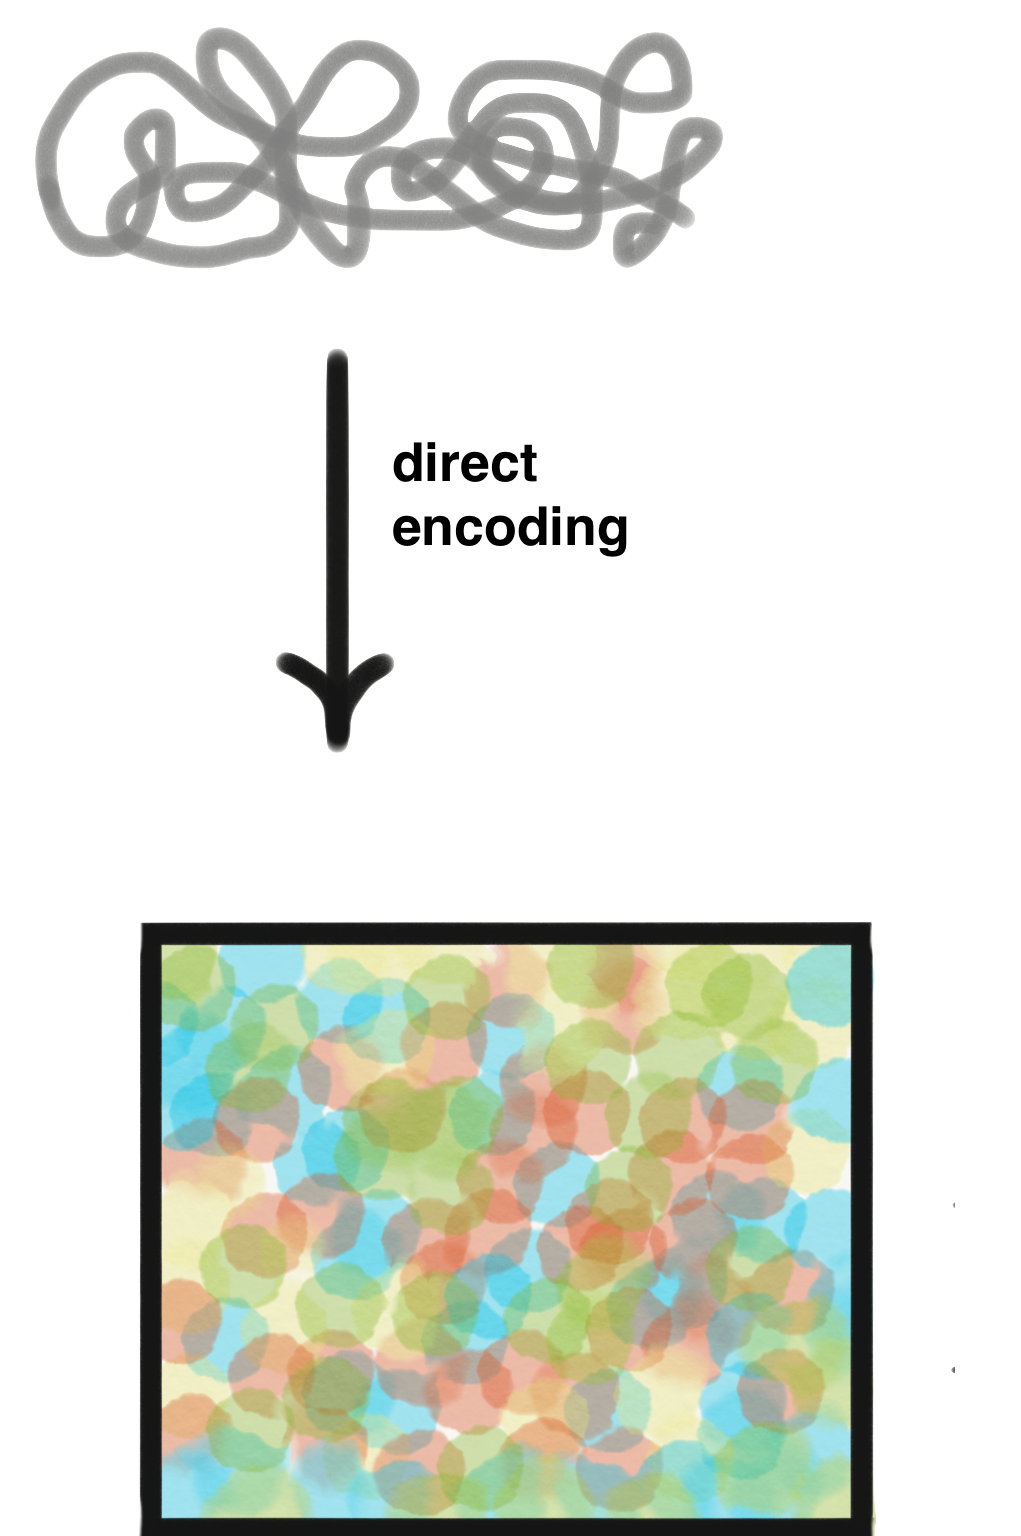
\includegraphics[width=\textwidth]{img/irregularity_direct_encoding.png}
        \caption{direct encoding}
        \label{subfig:direct_encoding}
    \end{subfigure}
    \hfill
    \begin{subfigure}[b]{0.4\textwidth}
        \centering
        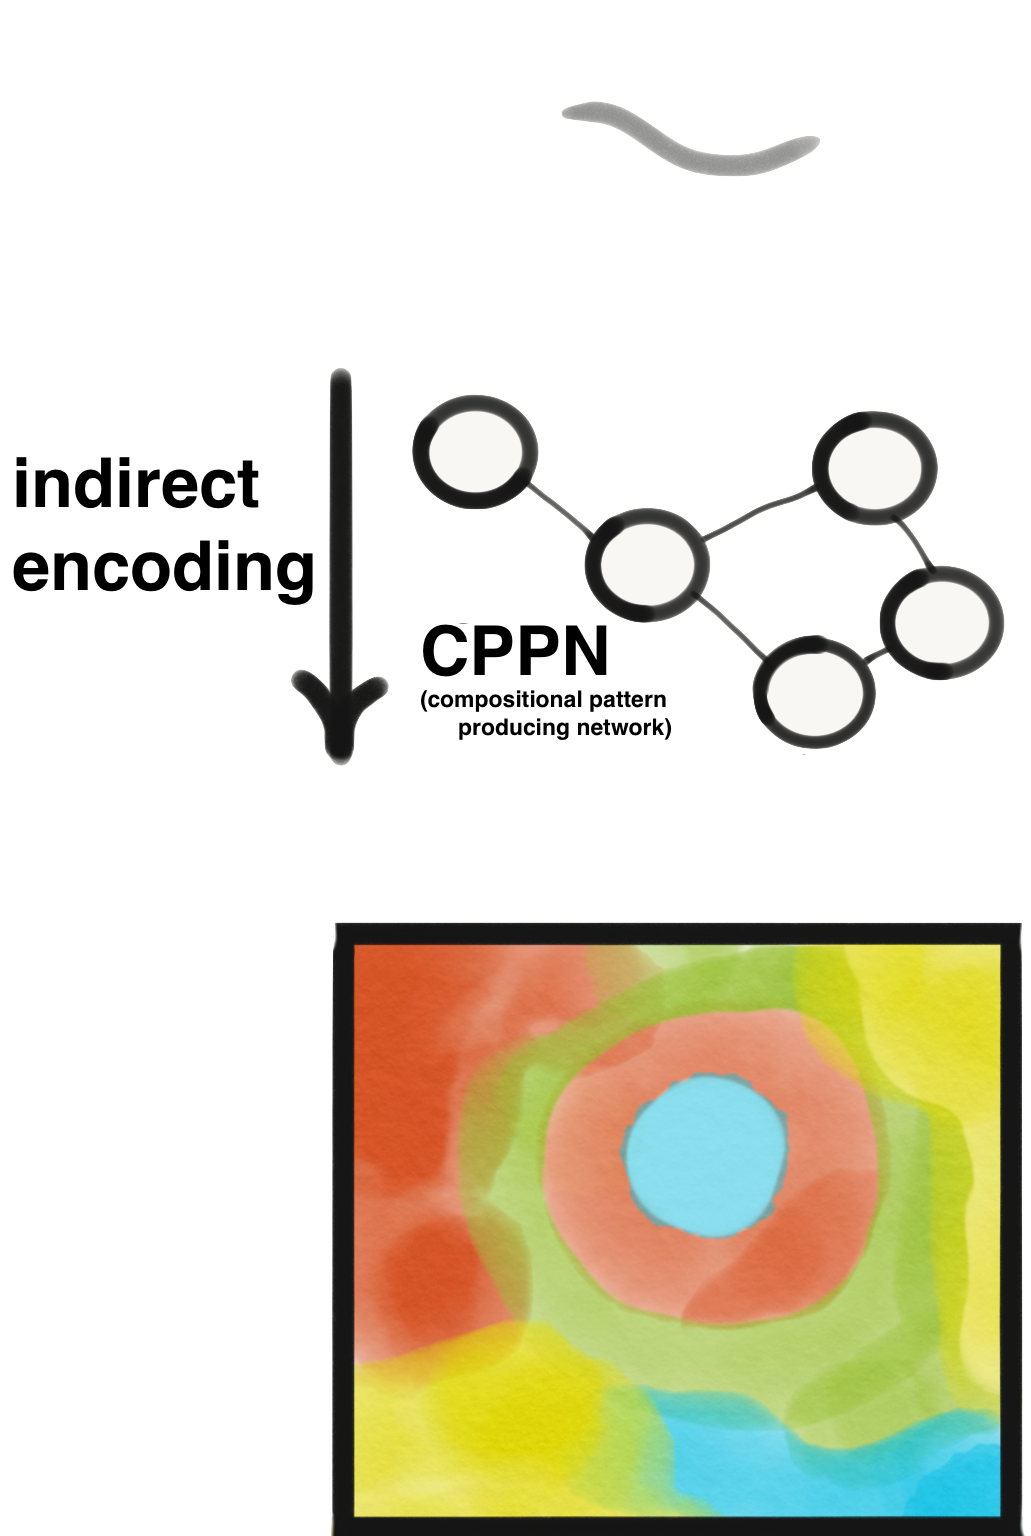
\includegraphics[width=\textwidth]{img/regular_indirect_encoding.png}
        \caption{indirect encoding}
        \label{subfig:indirect_encoding}
    \end{subfigure}
    \hfill
  \captionsetup{singlelinecheck=off,justification=raggedright}
  \caption{Archetypal examples of genotype to phenotype mapping from direct genetic representations and indirect phenotypic representations are illustrated. In both depictions, genetic information is shown at the top of the image and the corresponding phenotype is shown on the bottom of the image. In subfigure \ref{subfig:direct_encoding}, which depicts a direct encoding, a large volume of genetic information (where each characteristic of the phenotype is explicitly and independently described) is directly translated into a phenotype. Subfigure \ref{subfig:indirect_encoding} depicts an indirect encoding. In this particular scheme, a small amount of genetic information describes the configuration of a compositional pattern producing network (CPPN). This CPPN is then used to generate a phenotype. Indirect encodings are generally biased towards phenotypic regularity because phenotypic information is generated from a smaller amount of genetic information via a process that allows for multiple phenotypic elements to be determined by processes that tend to favor regularity and allows for genetic information to be reused to describe different components of the phenotype  \cite{Clune2011OnRegularity}.}
  \label{fig:indirect_bias}
\end{figure}

\begin{figure}[!htbp]
  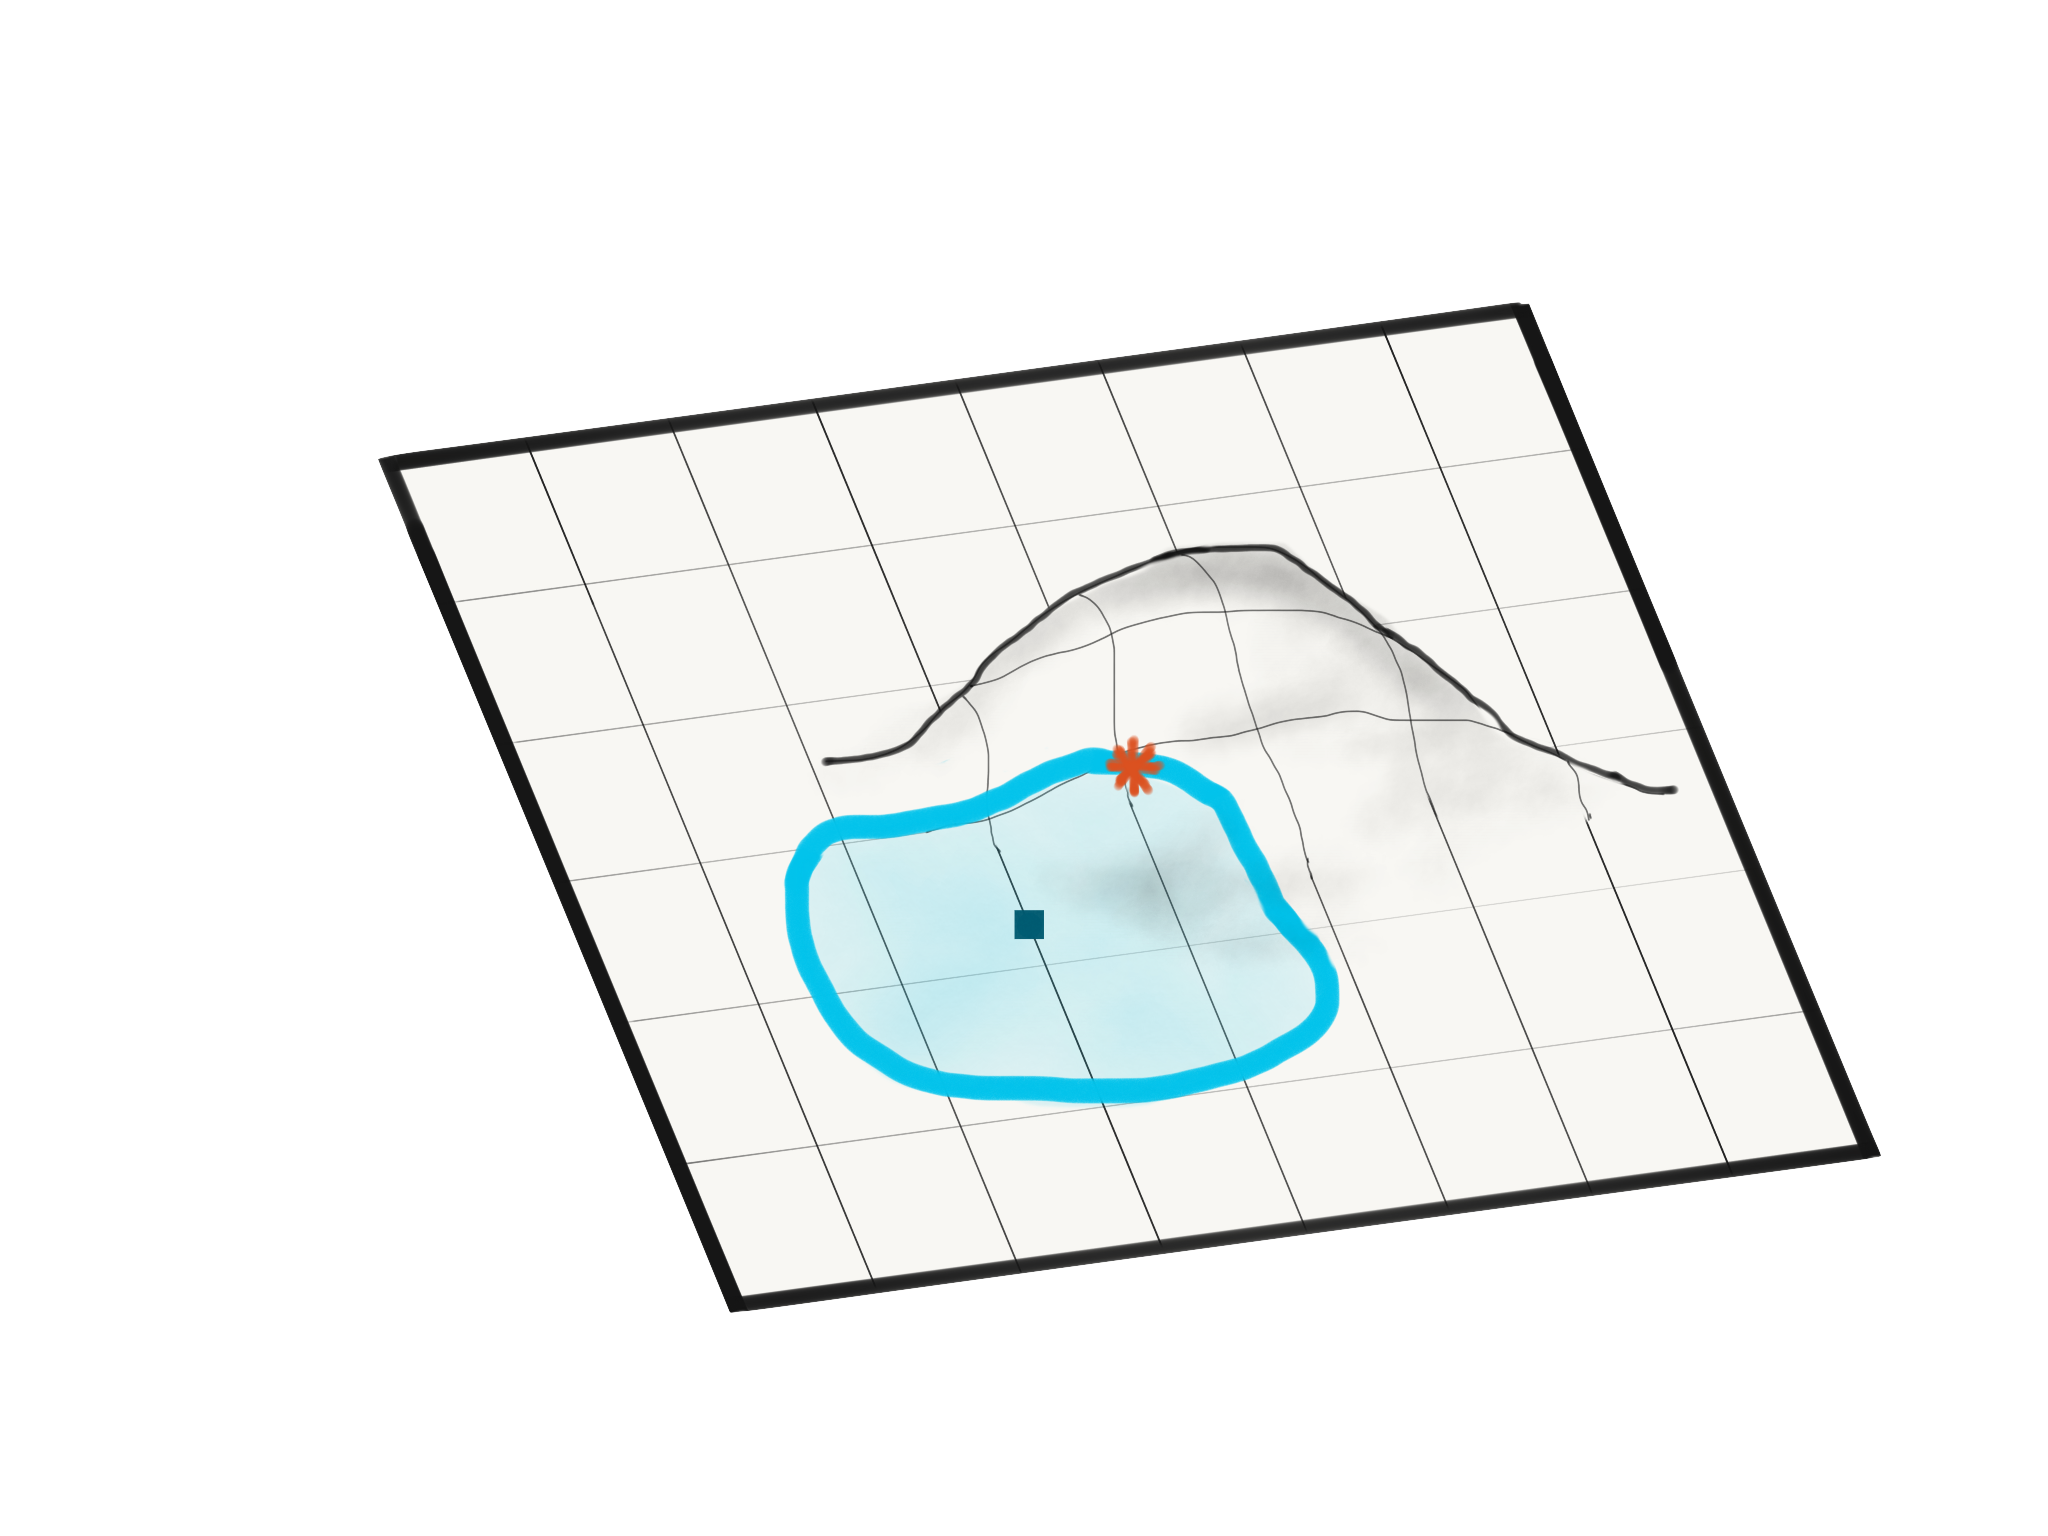
\includegraphics[width=0.8\textwidth]{img/baldwin_effect.png}
  \captionsetup{singlelinecheck=off,justification=raggedright}
  \caption{The Baldwin effect postulates that learning --- in evolutionary terms phenotypic plasticity or, equivalently and more explicitly, local search in the phenotype space --- biases evolutionary search to allow advantageous phenotypic features originally acquired via phenotypic plasticity to encoded into the genetic representation \cite{Downing2010TheNetworks}. In the first phase of the Baldwin effect, advantageous phenotypic features discovered by local search in the phenotype space increase the fitness of individuals proximal to that phenotype. Phenotypic plasticity is illustrated in the above cartoon, where the phenotype space is depicted as a three dimensional surface with points on the surface representing different phenotypes and the height of the surface denoting the fitness of the phenotypes at those points. In the illustration, the dark blue square represents the phenotype originally mapped to by the genetic representation of an individual, the blue shaded region represents the region of the phenotype space searched via phenotypic plasticity, and the red star represents a high fitness phenotypic variant reached via phenotypic plasticity. The fitness boost gained from phenotypic proximity to a high fitness solution biases evolutionary search to continue exploring that region of the instead of proceeding in other directions. In the second phase of the Baldwin effect, that continued evolutionary search promotes phenotypic features discovered by phenotypic plasticity are encoded into the genetic representation. Cost or unreliability of generating the advantageous phenotypic feature via phenotypic plasticity provides evolutionary pressure that favors genetic encoding of that phenotypic feature. In the case of indirect genotype to phenotype mappings, a direct genetic encoding of the feature discovered via phenotypic plasticity might not exist; however, genomes that map to phenotypes closer to the phenotypic feature discovered by plasticity --- which support attainment of the phenotypic feature by reducing the cost or increasing the reliability of acquiring that feature via plasticity, providing ``scaffolding'' for the local phenotypic search --- may still arise and will be selected for \cite{DowningHeterochronousBaldwinism}.}
     \label{fig:baldwin_effect}
\end{figure}

\begin{figure}[!htbp]
 \centering
    \begin{subfigure}[b]{0.5\textwidth}
        \centering
    	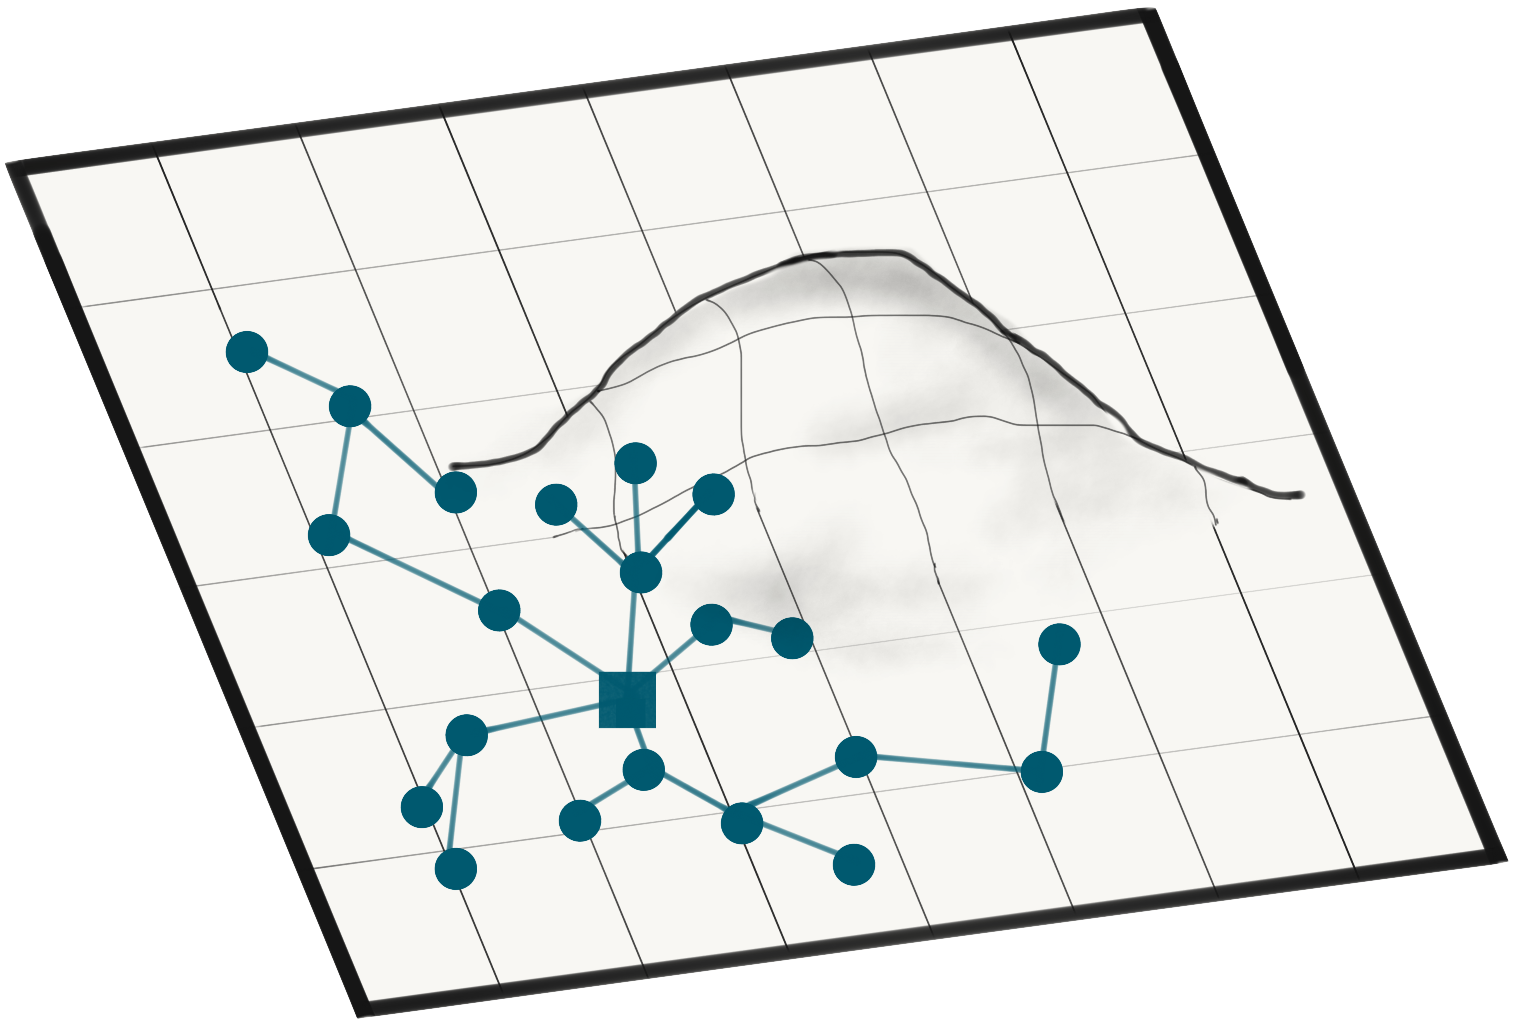
\includegraphics[width=\textwidth]{img/slow_cooling.png}
        \caption{slow cooling rate}
        \label{subfig:slow_cooling}
    \end{subfigure}%
    \hfill
    \begin{subfigure}[b]{0.5\textwidth}
        \centering
        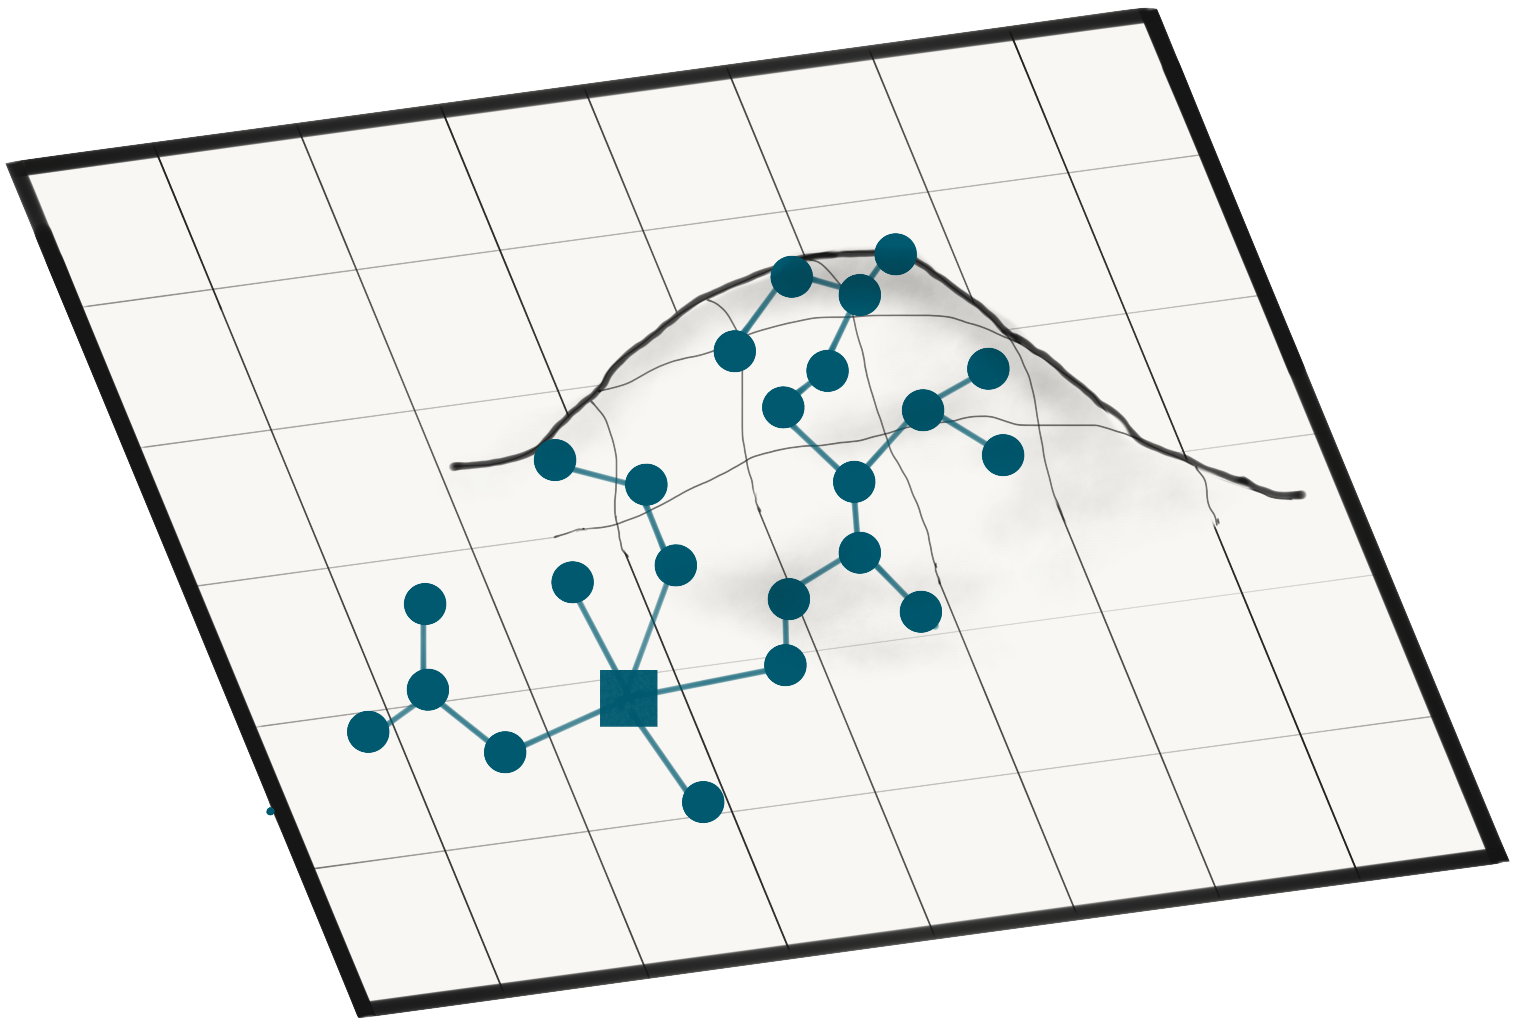
\includegraphics[width=\textwidth]{img/medium_cooling.png}
        \caption{medium cooling rate}
        \label{subfig:slow_cooling}
    \end{subfigure}
    \hfill
    \begin{subfigure}[b]{0.5\textwidth}
        \centering
        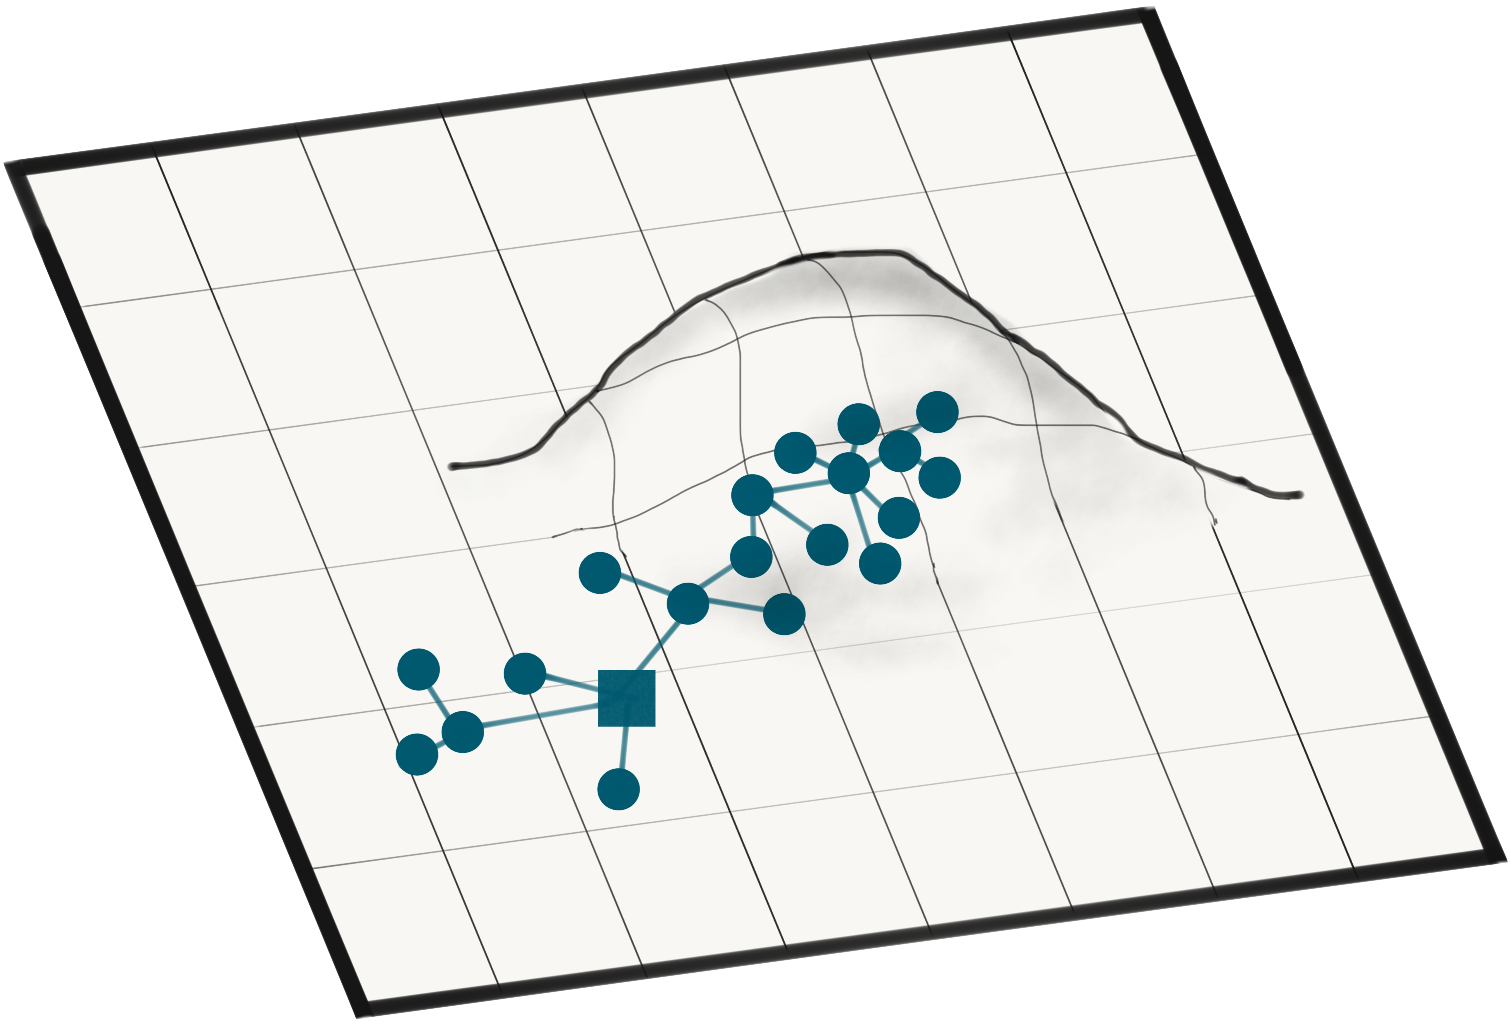
\includegraphics[width=\textwidth]{img/fast_cooling.png}
        \caption{fast cooling rate}
        \label{subfig:fast_cooling}
    \end{subfigure}
 	\captionsetup{singlelinecheck=off,justification=raggedright}
    \vspace{-2ex}
  \captionsetup{singlelinecheck=off,justification=raggedright}
  \caption{The three modes of local phenotype space search proposed are illustrated. In each illustration, the phenotype space is depicted as a three dimensional surface with points on the surface representing different phenotypes and the height of the surface denoting the fitness of the phenotypes at those points. The original phenotype mapped to by a genetic representation is shown with a square. Points marked with a circle denote phenotypes explored during the local search processes. Lines connecting the points represent that one point was reached from the other by a mutation of the direct representation of a phenotype. Subfigure \ref{subfig:static_mutation} depicts the direct mutation local phenotypic search process, where points explored are generated by mutations to the direct representation of the original phenotype mapped to by a genetic representation. Subfigure \ref{subfig:random_walk} depicts the random walk local phenotypic search process, where points explored are generated by mutation to the direct representation of the point explored immediately before (starting from the direct representation of the original phenotype mapped to by a genetic representation). Finally, subfigure \ref{subfig:simulated_annealing} depicts the simulated annealing local phenotypic search process, where points are explored via mutation to the direct representation of a randomly chosen point previously explored with an increasingly strong bias towards exploring from points with high fitness as the exploration process proceeds.}
  \label{fig:local_search_types}
\end{figure}

\begin{figure}[!htbp]

  \captionsetup{singlelinecheck=off,justification=raggedright}
  \caption{words}
  
\label{fig:evolutionary_algorithm}
\end{figure}

\clearpage
\printbibliography

%\section{Motivation}

While neural architectures with high potential for irregular refinement are highly desirable, directly selecting for irregular refinement potential by performing complete irregular refinement on all candidate solutions is computationally prohibitive.
In the spirit of the Baldiwn effect, I propose that local phenotypic search via mutation to the direct representation of candidate solutions could bias evolutionary search toward neural architectures with high potential for irregular refinement.
While experimental results validate the Baldwin hypothesis,\autocite{Downing2009ComputationalEffect} the type and degree of local phenotypic search necessary to meaningfully bias evolutionary search is unknown.
The proposed research will characterize evolutionary bias towards artificial neural architectures with high irregular refinement potential induced by varied methods of local phenotypic search, specifically considering (1) the organization of local phenotypic search, the degree to which that search is biased by distribution of fitness over the local phenotypic space, and (2) selective preference for characteristics of local phenotypic space, the degree to which the presence of fitness peaks is considered over the overall fitness of the local phenotypic neighborhood.
A better understanding of these questions will translate to methodology that promotes evolution of neural architectures highly conductive to irregular refinement as well as furthering the theoretical conception of the interplay between phenotypic plasticity and evolution.
 


%\section{Background}

Neuroevolution aims to design artificial neural network (ANN) topologies and weighting schemes through repeated evaluation, selection, and recombination of candidate solutions, an algorithm inspired by biological evolution. In the biological metaphor, candidate solutions have a phenotype, an ANN configuration that evolutionary selection acts upon, and a genotype, information that mutation and recombination act on and from which the phenotype is constructed. Genotypic representations are said to be either direct, indicating that each characteristic of the phenotype is stored verbatim in the genome, or indirect, indicating that the phenotype is generated from information that does not bear a one-to-one relationship to phenotypic characteristics. Direct mappings, which allow evolution to tweak individual phenotypic characteristics of candidate solutions independently, alllow fine-tooothed exploration of the phenotypic search space. Conversely, indirect genetic encodings, where genetic information is expanded via a process that allows for reuse of that information to uniformly describe a large number of phenotypic characteristics, has been demonstrated to bias evolutionary search towards phenotypic regularity\autocite{Clune2011OnRegularity}.

As a result of this bias, in highly regular problem domains evolutionary search with indirect genetic encoding outperforms search relying upon direct genetic encoding \autocite{Clune2011OnRegularity}. Nevertheless, most problem domains exhibit some irregularity, which often can only be exploited irregular phenotypic refinement; experimental evidence indicates that champion solutions evolved with indirect genetic encoding can often be bettered by irregular refinement vis-\`a-vis further evolutionary search with a direct encoding \autocite{Clune2011OnRegularity}. Clune et al. postulate that learning (post-developmental phenotypic plasticity of a neural network) similarly constitutes irregular refinement, enhancing the performance of a highly regular indirectly encoded phenotype via irregular modifications. Further, by allowing a candidate solution to assume proximal phenotypic forms, learning enables evolutionary selection to act on information about a candidate solution's local phenotypic neighborhood. Through selective pressure for phenotypes proximal to high-fitness phenotypic forms, local phenotypic search ``buys evolutionary time'' until heritable scaffolding arises to support phenotypic adaptation originally attained via plasticity \autocite{Downing2010TheNetworks}. This concept is termed the Baldwin effect.

%\section{Topic}

 This project will focus on Evolving Artificial Neural Networks (EANN), a widely-explored alternative to back-propagation paradigm of network trainingThis project will focus on Evolving Artificial Neural Networks (EANN), a widely-explored alternative to back-propagation paradigm of network training \cite{DowningIntelligenceSystems}. While capable of generating recurrent structures and not requiring supervised learning during the training process, this approach can be stymied by its own set of challenges. In particular, designing these systems to be highly evolvable -- e.g., making them compatible with the evolutionary process by avoiding excessive fatal mutations and premature dead-end local maxima in the search space, for instance -- is a non-trivial task (especially for large networks). It is thought that moving beyond direct encodings where each topological connection and weight is explicitly specified, to adaptive, implicit, or generative genotype-phenotype mappings might address these issues. Promising research has been conducted in this vein. A prime example is the Genetic Regulatory Network (GRN) scheme of Reisinger and Miikkulainen, which they found yielded a more compact representation, more adaptive variation, and more robustness to mutation compared to the direct encoding (as well as alternate encodings) \cite{ReisingerAcquiringRepresentations}. This GRN scheme is just one of a number of genotype-phenotype mappings that have been explored, such as Neuroevolution of Augmenting Topologies (NEAT), cellular encoding (CE), and encodings based on context-free grammars \cite{DowningIntelligenceSystems}.



\end{document}